\documentclass[a4paper, 11pt]{report}

\usepackage[utf8]{inputenc}
\usepackage[francais]{babel}
\usepackage[T1]{fontenc}
\usepackage[final]{pdfpages}
\usepackage{graphicx}
\usepackage{parskip}
\usepackage{hyperref}
\usepackage{subfig}

%\setlength{\parindent}{0.7cm}

\title{Éco-conception de logiciels\\ \large Rapport de stage de 5ème année}
\author{Guillaume Delamare}
\date{\today}

\begin{document}
\renewcommand{\labelitemi}{$\bullet$}
\renewcommand{\labelitemii}{$\diamond$}
\renewcommand{\labelitemiii}{$\ast$}
\renewcommand{\labelitemiv}{$\cdot$}

%TODO faire la page de garde
\maketitle

\section*{Remerciement}
%TODO Relire les remerciement
Je tiens, tout d'abord, à remercier mon tuteur, Thomas Ledoux, pour m'avoir offert l'opportunité de travailler au sein de l'équipe ASCOLA. Je le remercie d'autant plus pour l'apport d'expérience et la richesse des situations dans lesquelles il me permet de travailler.

Je souhaite ensuite remercier Rémi Sharrock, pour sa bonne humeur et son aide précieuse tout au long de mon travail, ainsi que, l'ensemble des membres de l'équipe ASCOLA et du département d'informatique de l'école des Mines de Nantes pour leurs accueils, leurs aides et leurs conseils.

Je remercie aussi mon encadrant, Benoit Parrein, pour l'aide et le suivi tout au long de cet exercice qu'est le stage de fin d'étude. Et pour finir je souhaite remercier Polytech Nantes, dans son ensemble, pour les trois années de formation et d'encadrement dont j'ai pu profiter.

\newpage

\section*{Résumé}
%TODO écrire le résumé

\newpage

\tableofcontents

\chapter{Introduction}
%TODO écrire l'introduction
% Contexte de la rédaction de ce document
% Préssentation du plan

\chapter{Présentation du stage}
%TODO Relire le chapitre Présentation du stage
	\section{Présentation du lieu de stage}
Mon stage de cinquième année se déroule au sein de l’équipe ASCOLA du laboratoire LINA dans les locaux de l’école des Mines de Nantes.
		\subsection{L'école des Mines de Nantes}
L’école des Mines de Nantes (EMN) est une école d’ingénieur française sous tutelle du ministère de l’industrie. L’école est rattachée à l’institut Mines-Télécom, au Groupe des écoles des Mines et à la Conférence des grandes écoles.

Elle a été créée en 1990 sur le site de la Chantrerie à Nantes et accueille 850 élèves ingénieurs en formation initiale. Le recrutement est effectué par concours après deux années de classe préparatoire. En 2011, l’EMN a décerné 250 diplômes d’ingénieur.

L’école est séparée en 5 départements axé sur les thématiques des équipes de recherche de l'école. On dénombre les départements :
\begin{itemize}
	\item D'informatique
	\item D'automatique et productique (DAP)
	\item De systèmes énergétiques et environnement (DSEE)
	\item De physique subatomique et technologies associées (Subatech)
	\item De sciences sociales et de gestion (DSSG)
\end{itemize}

		\subsection{L'équipe de Recherche}
Mon stage se déroule dans l'équipe ASCOLA. Cette équipe est installée au sein du département informatique de l’EMN au côté de l'équipe TASK. L'équipe ASCOLA fait partie du LINA (Laboratoire d'Informatique de Nantes Atlantique) ainsi que de l'INRIA (Institut National de Recherche en Informatique et en Automatique).

Cette équipe regroupe une trentaine de personnes qui travaillent sur les langages d'aspects et de composition. Les axes de recherche, tel qu'ils le sont présentés sur la page dédié à l'équipe ASCOLA sur le site de l'INRIA\footnote{\href{http://www.inria.fr/equipes/ascola}{www.inria.fr/equipes/ascola}}, sont :
\begin{itemize}
	\item le développement de nouveaux concepts, de support linguistique, et d'outils pour les applications distribuées permettant de gérer notamment les préoccupations transverses comme la distribution elle-même, les comportements transactionnels et la sécurité ;
	\item la définition d'un modèle qui intègre de manière transparente composants et aspects, en particulier au travers d'une notion d'interface rendant possible le découplage des composants et des aspects concrets, tout en permettant l'analyse et l'application de propriétés de composition dans un contexte hybride composant/aspect ;
	\item l'investigation des relations entre langages dédiés, langages d'aspects et langages de composition. Nous comptons exploiter les similitudes entre ces classes de langages dans le cadre du développement de techniques de conception et d'implémentation des langages de manière à faciliter un développement par transformations d'applications efficaces et correctes à partir d'abstraction de programmation de haut niveau ;
	\item l'étude des fondements de la programmation par aspects et de leurs propriétés de composition au moyen de sémantiques formelles pour les aspects (et les composants) ainsi que des techniques d'analyse, de vérification et de validation correspondantes.
\end{itemize}

Mon stage se déroule sous la tutelle de Thomas Ledoux qui, avec Jean Marc Menaud, Adrien Lèbre, Rémi Sharrock, ainsi que leurs doctorants, travaille sur des aspects cloud computing, virtualisation et écologie des systèmes d'informations.

	\section{Présentation du sujet de stage}
Dans cette partie je vais décrire ce qu'est dans la pratique mon sujet de stage. Je joins en annexe le document original de sujet de stage tel qu'il été écrit au moment de la signature de ma convention.

		\subsection{Contexte}
Mon stage se positionne dans les travaux GreenIT de l’équipe ASCOLA. Je travaille donc principalement avec la sous-partie de l'équipe qui effectue de la recherche dans ce domaine là. L'équipe travaille déja sur diférant projet portant sur le cloud computing, la virtualisation avec en dénominateur commun le GreenIT. On peut citer par exemple des travaux sur la migration à chaud de machine virtuelle qui donné lieu à la création de la startup easyVirt.

L'équipe travail aussi sur d'autre travaux comme %TODO finir le paragraphe

		\subsection{Sujet}
De nos jour, l'informatique est omniprésent. Que ce soit au travail, à la maison, dans nos manières de nous documenté comme dans nos façons de produire, nous utilisons l'outil informatique. Cette informatique est devenu au fil des années de plus en plus gourmande en énergie. La multiplication des réseaux, des centres de données, des terminaux pour se raccorder au système, tout ceci demande toujours plus d'énergie.

Actuellement des efforts sont fait pour optimiser la couche matérielle afin de la rendre toujours plus efficace. Seulement ce n'est pas suffisant. Afin de limiter l'augmentation certaine de la consommation d'énergie des équipements informatique, il faut aussi s'attaquer à la source de ce besoin d'énergie, le logiciel. C'est lui, en effet qui a besoin d'effectuer des calcule, des entrées/sorties, des communications réseaux qui font consommer le matériel.

Des travaux ont bien mis en évidence que, les choix fait lors de la conception d'un logiciel, peuvent être déterminant par rapport à la consommation de celui ci. Ces choix sont divers et variés. Il peut s'agir de la technologie utilisé, mais aussi de l'architecture choisie pour le logiciel ou encore de l'environnement dans lequel ce logiciel fonctionne.

Le sujet de ce stage est donc de proposer, d'étudier et de valider par l'expériementation un certain nombre de suggestions qui permettraient de réduire l'emprunte énergétique d'un logiciel.

		\subsection{Objectifs}
Le Sujet de mon stage est donc l'éco-conception de logiciel. Il s'agit d'étudier les différentes pistes qui s'ouvrent à nous pour rendre plus écologique les systèmes d'informations en jouant sur la composante logicielle de ceci. Mon travail est donc de plusieurs ordres.

Je dois tout d'abords rechercher les travaux existants dans ce domaine, qu'il soit centré sur l'éco-conception ou bien positionné sur des domaines anexes comme l'analyse de codes ou bien le cycle de vie du logiciel. Suite à ça, je devrais élaborer un certain nombre de propositions de contribution afin de centrer mon travail à venir. Enfin je devrais expérimenter et valider mes résultats afin de pouvoir emmètre des recommandations en terme d'éco-conception.

Deux travaux transversaux sont à effectuer. Premièrement je dois étudier et mettre en place une méthodologie permettant d'évaluer l'efficacité énergétique d'un code.

\chapter{État de l'art}
	\section{Introduction}
	% TODO Ecrire l'introduction de l'état de l'art
		\subsection{Pourquoi économiser de l'énergie}

		
		\subsection{L'éco-conception : définition}
			\subsubsection{L'analyse du cycle de vie}
			
		
	\section{La mesure de consommation d'énergie}
	%TODO Finir d'écrire la section sur la mesure de cosommation
		\subsection{Différentes approches pour mesurer la consommation des ressources}
			\subsubsection{La mesure par un appareil externe}
La première méthodes, la plus commune pour mesurer les resources consommées par un appareil électrique, est de placer un wattmètre en série sur l'alimentation de cet appareil. Avec un wattmètre récent on peut mesurer un ensemble de paramètre tel que les watts, les watts/heure, les volts et les ampères. De plus la plupart des outils récent propose un système d'enregistrement et/ou de transfert des données vers un ordinateur.

Par exemple, les \textit{plugwizes} sont des modules qui se placent sur la prise. sont capable de couper l'alimentation de l'appareil branché dessus et de mesurer la consommation électrique de celui ci. Ils sont capable de transmètre ces informations sans fils jusqu'à un ordinateur. Un autre exemple de ce type de matériel, les wattmètres de la marque \textit{watts up\/?}. Ils permettent, suivant leur gamme, de collecter de l'information et de la transmètre. Le \textit{watts up\/? pro .net} (figure~\ref{wattsUp}) dispose d'un système d'enregitrement de, au maximum, 120000 mesures de watts et de deux interface de communication, USB et Ethernet.

\begin{figure}
	\begin{center}
		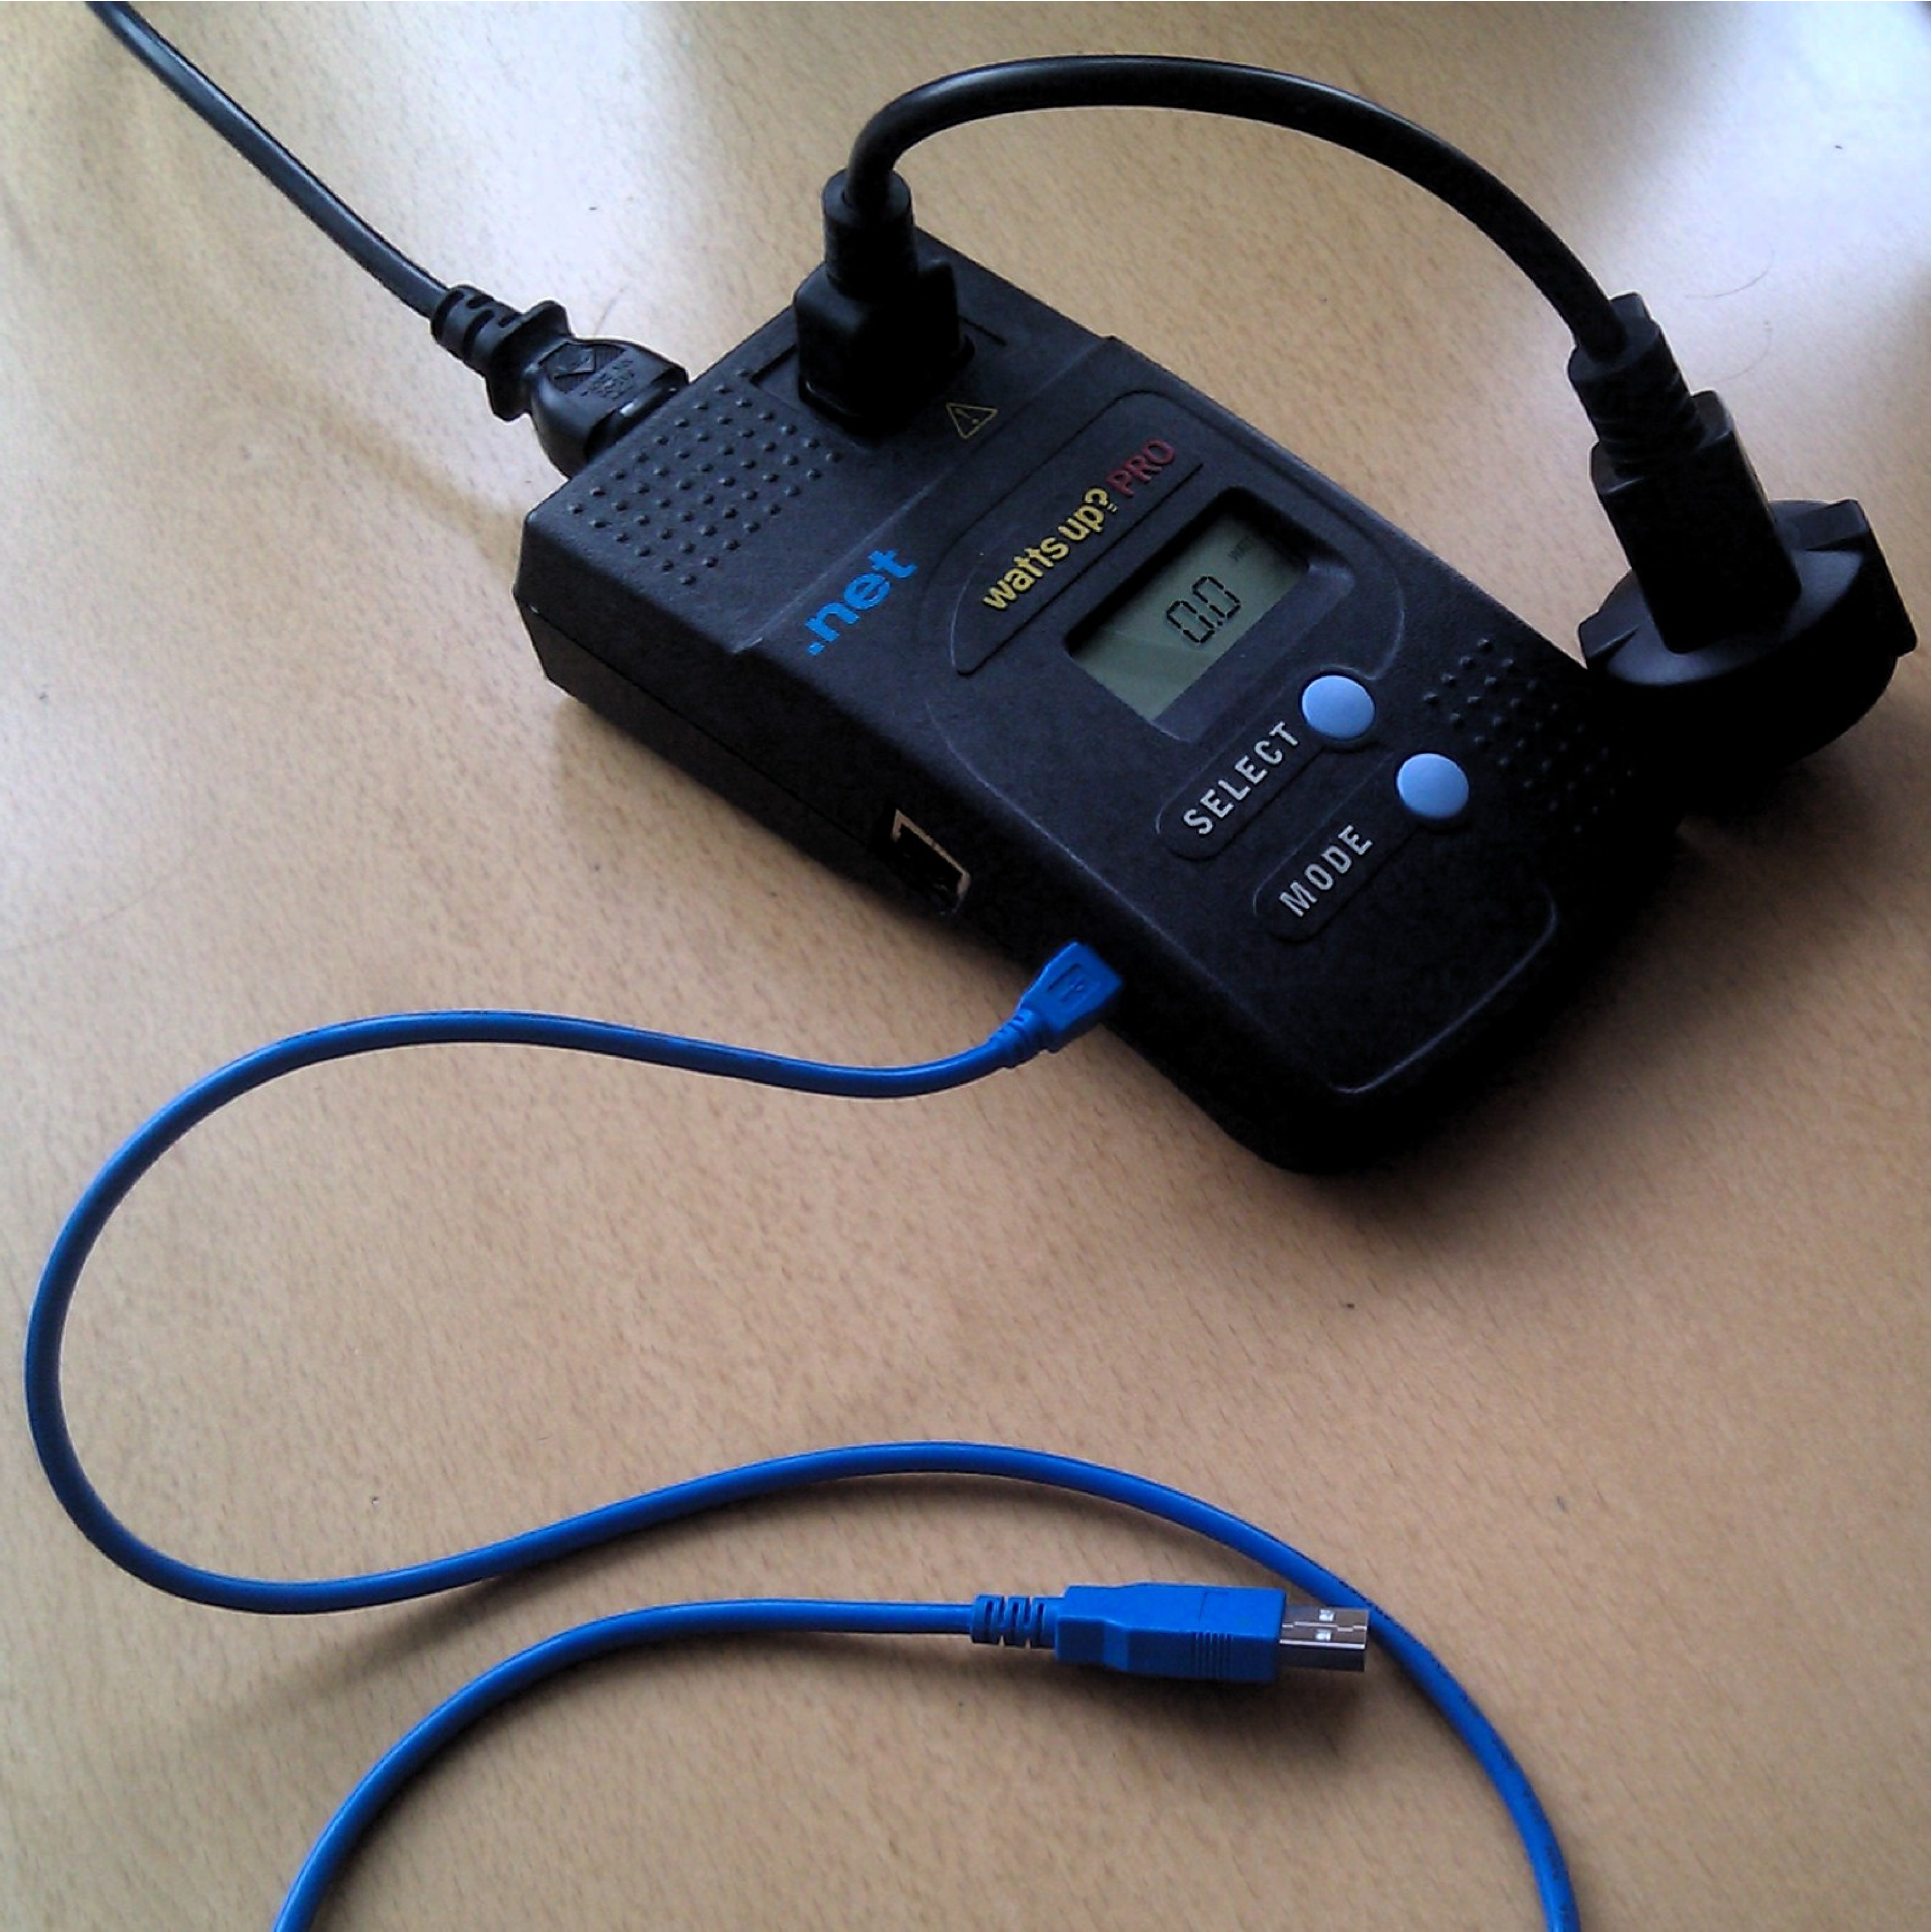
\includegraphics[width=7cm,height=7cm]{figures/wattsUp.eps}
		\caption{Photo d'un wattmètre watts up pro .net}
		\label{wattsUp}
	\end{center}
\end{figure}

Cette technique de mesure n'offre qu'une vu global de notre système. Il est impossible par cette méthode d'identifier de manière certaine la consommation d'un logiciel. On peut par contre corréler un changement de consommation avec un événement survenu (le démarage d'une application, le lancement d'une tache gourmande en traitement\ldots). 

			\subsubsection{La mesure par un logiciel interne}
La deuxième méthode consiste à analyser les ressources utiliser par un programme et, à partir d'un modèle de consommation, d'en déduire la consommation énergétique de l'application. Différentes ressources peuvent être ciblées. On peut les classer en deux catégories : les unités de calcul (CPU, GPU\ldots) et les dispositifs d'entrées/sorties (disque dur, interface réseau\ldots).

Pour les unités de calcul, deux modèles sont possible pour extraire une consommation. On peut soit utiliser le pourcentage d'utilisation par l'application de l'unité, soit utiliser le temps 

référence à cet article \cite{noureddine:hal-00681560}

			\subsubsection{Vers une mesure par un appareil interne}
Le future !!! des wattmètres/des sondes installer dans chaque composant. référernce à cet article\cite{Esmaeilzadeh:2011:LBL:1950365.1950402}
		
		\subsection{Comment comparer la consommation de deux logiciels}
			\subsubsection{Deux versions d'un logiciel}
Article Green mining\cite{GreenMining} décrivant une méthodologie

			\subsubsection{Deux logiciels isofonctionnel}
Parler des métriques.

			\subsubsection{Deux logiciels diférents}
Parler de métrique plus complexe.
		
	\section{Fabriquer un éco-logiciel}
	%TODO Ecrire la section Fabriquer un eco-logiciel
		\subsection{De la Conception\ldots}
		
		\subsection{\ldots à la programmation}
		
		\subsection{La programmation Modulaire}
			\subsubsection{Intéret de la programmation modulaire dans l'économie d'énergie}
			\subsubsection{OSGi : du java modulaire}
		
		
		
	\section{Travaux similaire}
	%TODO Ecrire la section Travaux similaire
		\subsection{Le Green code Lab}
		\subsection{Le projet code vert}
		
	\section{Conclusion}
	%TODO Ecrire la section Conclusion de l'état de l'art

\chapter{Comment peut on mesurer la consommation d'un logiciel ?}
%TODO écrire le chapitre Comment peut on mesurer la consommation d'un logiciel
	\section{Qu'est ce qui consomme dans un ordinateur ?}
	\section{Outils de mesure de la consommation des ressources par un logiciel}

\chapter{Mise en valeur de l'impact du code sur la consommation}
%TODO écrire le chapitre Mise en valeur de l'impact du code sur la consommation
	\section{Impact du choix du langage}
	\section{Impact des choix de programmation}
		\subsection{Description des tests}
		\subsection{Resultats obtenus}

\chapter{La programmation modulaire au service de l'économie d'énergie}
%TODO écrire le chapitre La programmation modulaire au service de l'économie d'énergie
Afin de mettre en valeur l'importance de l'architecture logiciel dans la consommation, j'ai proposé de développer une application basé sur la technologie java OSGi\footnote{\href{http://www.osgi.org}{www.osgi.org}}. L'objectif de ce projet est de pouvoir réaliser facilement des démonstrations d'application modulaire qui s'adapte en fonction de contrainte énergétique. J'ai donc choisi d'élaborer un quadriciel qui permettrai d'échanger une partie de l'application (dans notre context un bundle OSGi) contre une autre afin d'optimiser la consommation.

Un cas d'utilisation abstrait de cet application serait qu'un programme réalise une tache. Le développeur connait deux algorithmes pour coder cette tache. Ils ont chacun leurs forces et leurs faiblesses.

\begin{figure}[htp]
  \centering
  \subfloat[Courbe de consommation du bundle A]{\label{AbsBdlA}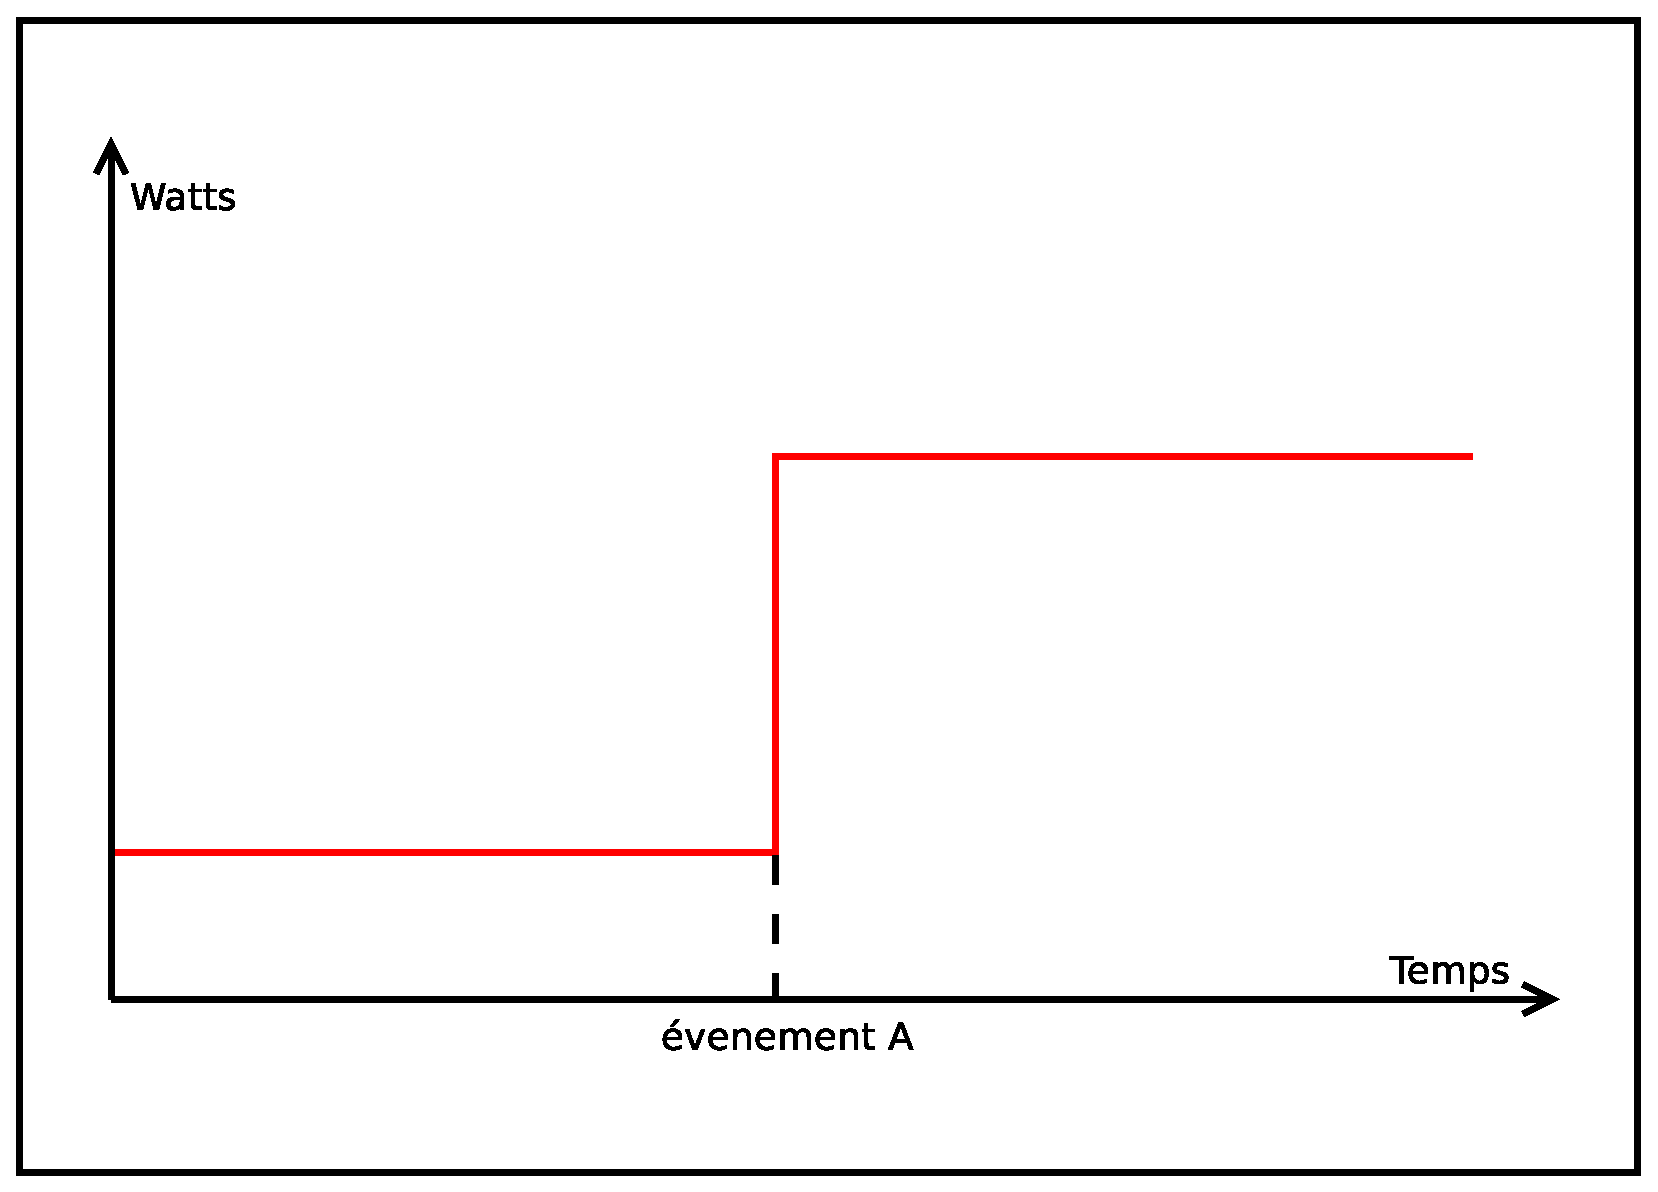
\includegraphics[width=5cm]{figures/Abstract_bundle_A.eps}}                
  \subfloat[Courbe de consommation du bundle B]{\label{AbsBdlB}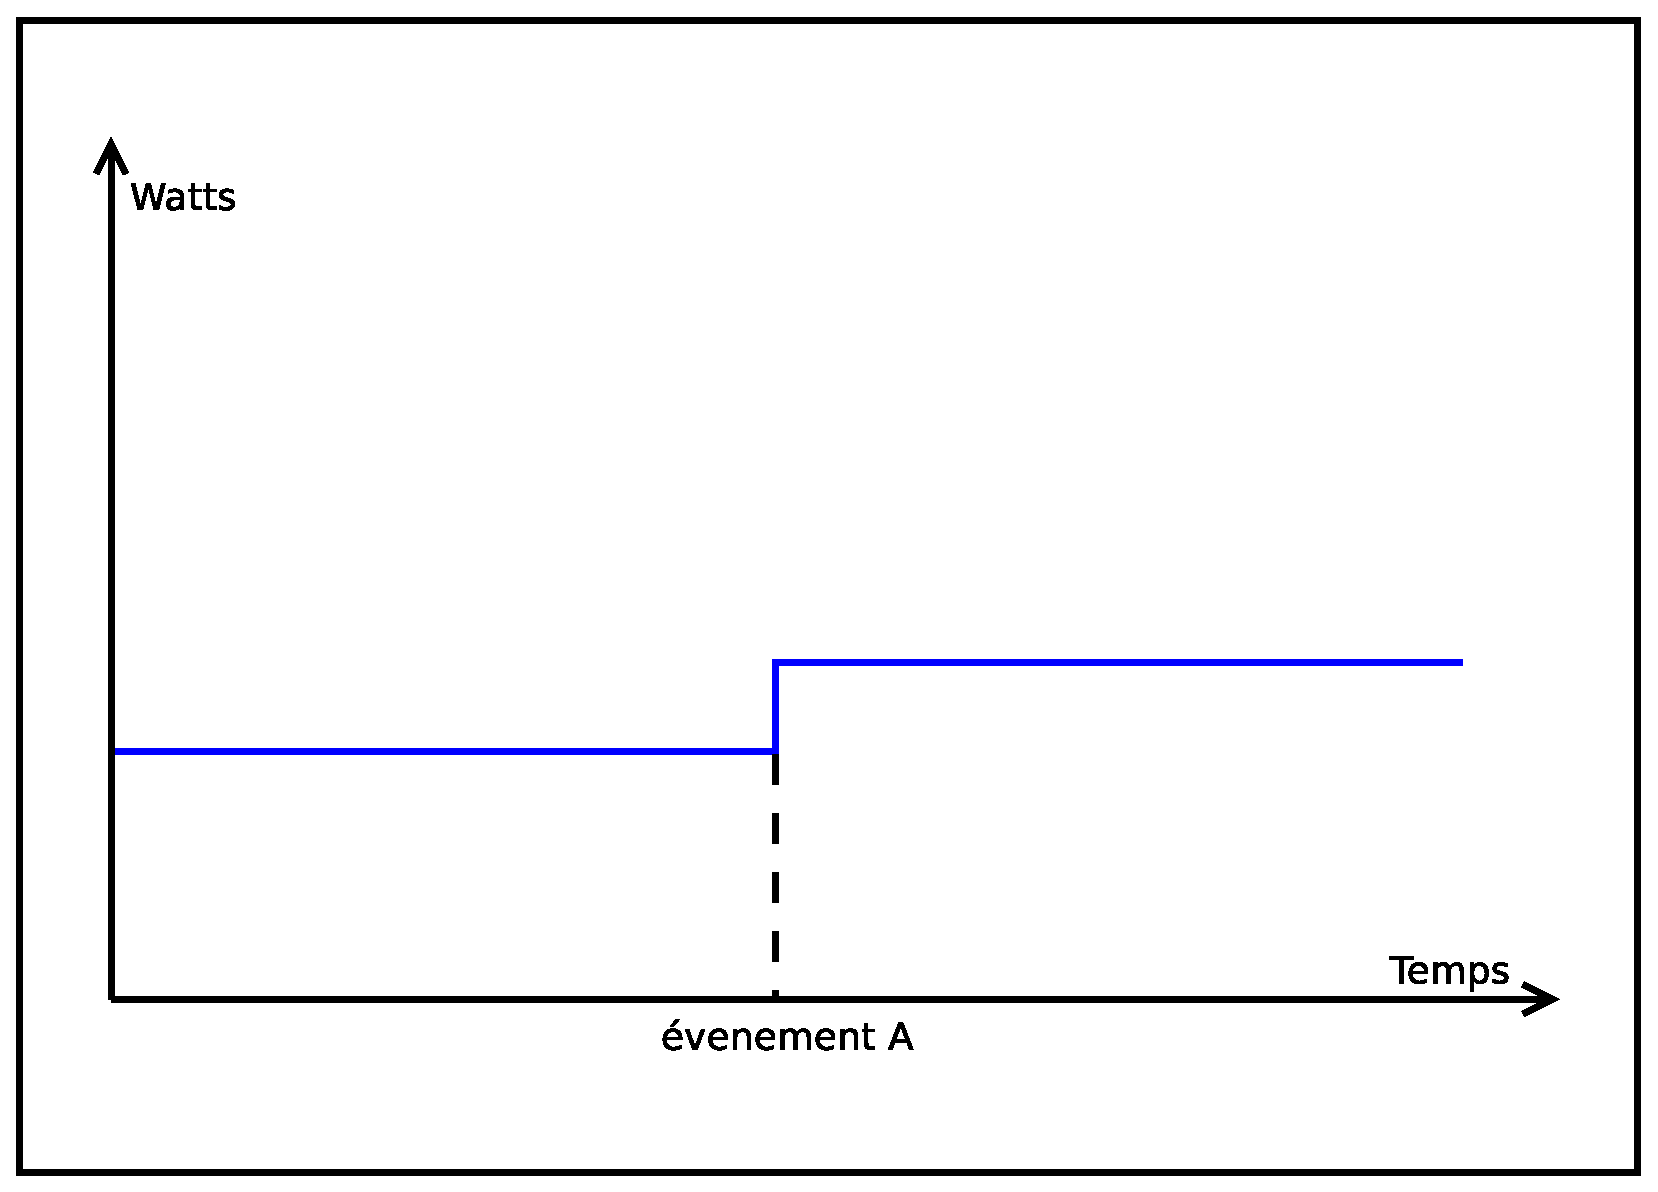
\includegraphics[width=5cm]{figures/Abstract_bundle_B.eps}}
  \caption{Illustration de l'optimisation de la consommation par l'échange de bundle}
  \label{AbsBdl}
\end{figure}

	\section{Présentation de l'infrastructure développé}
\begin{figure}
	\begin{center}
		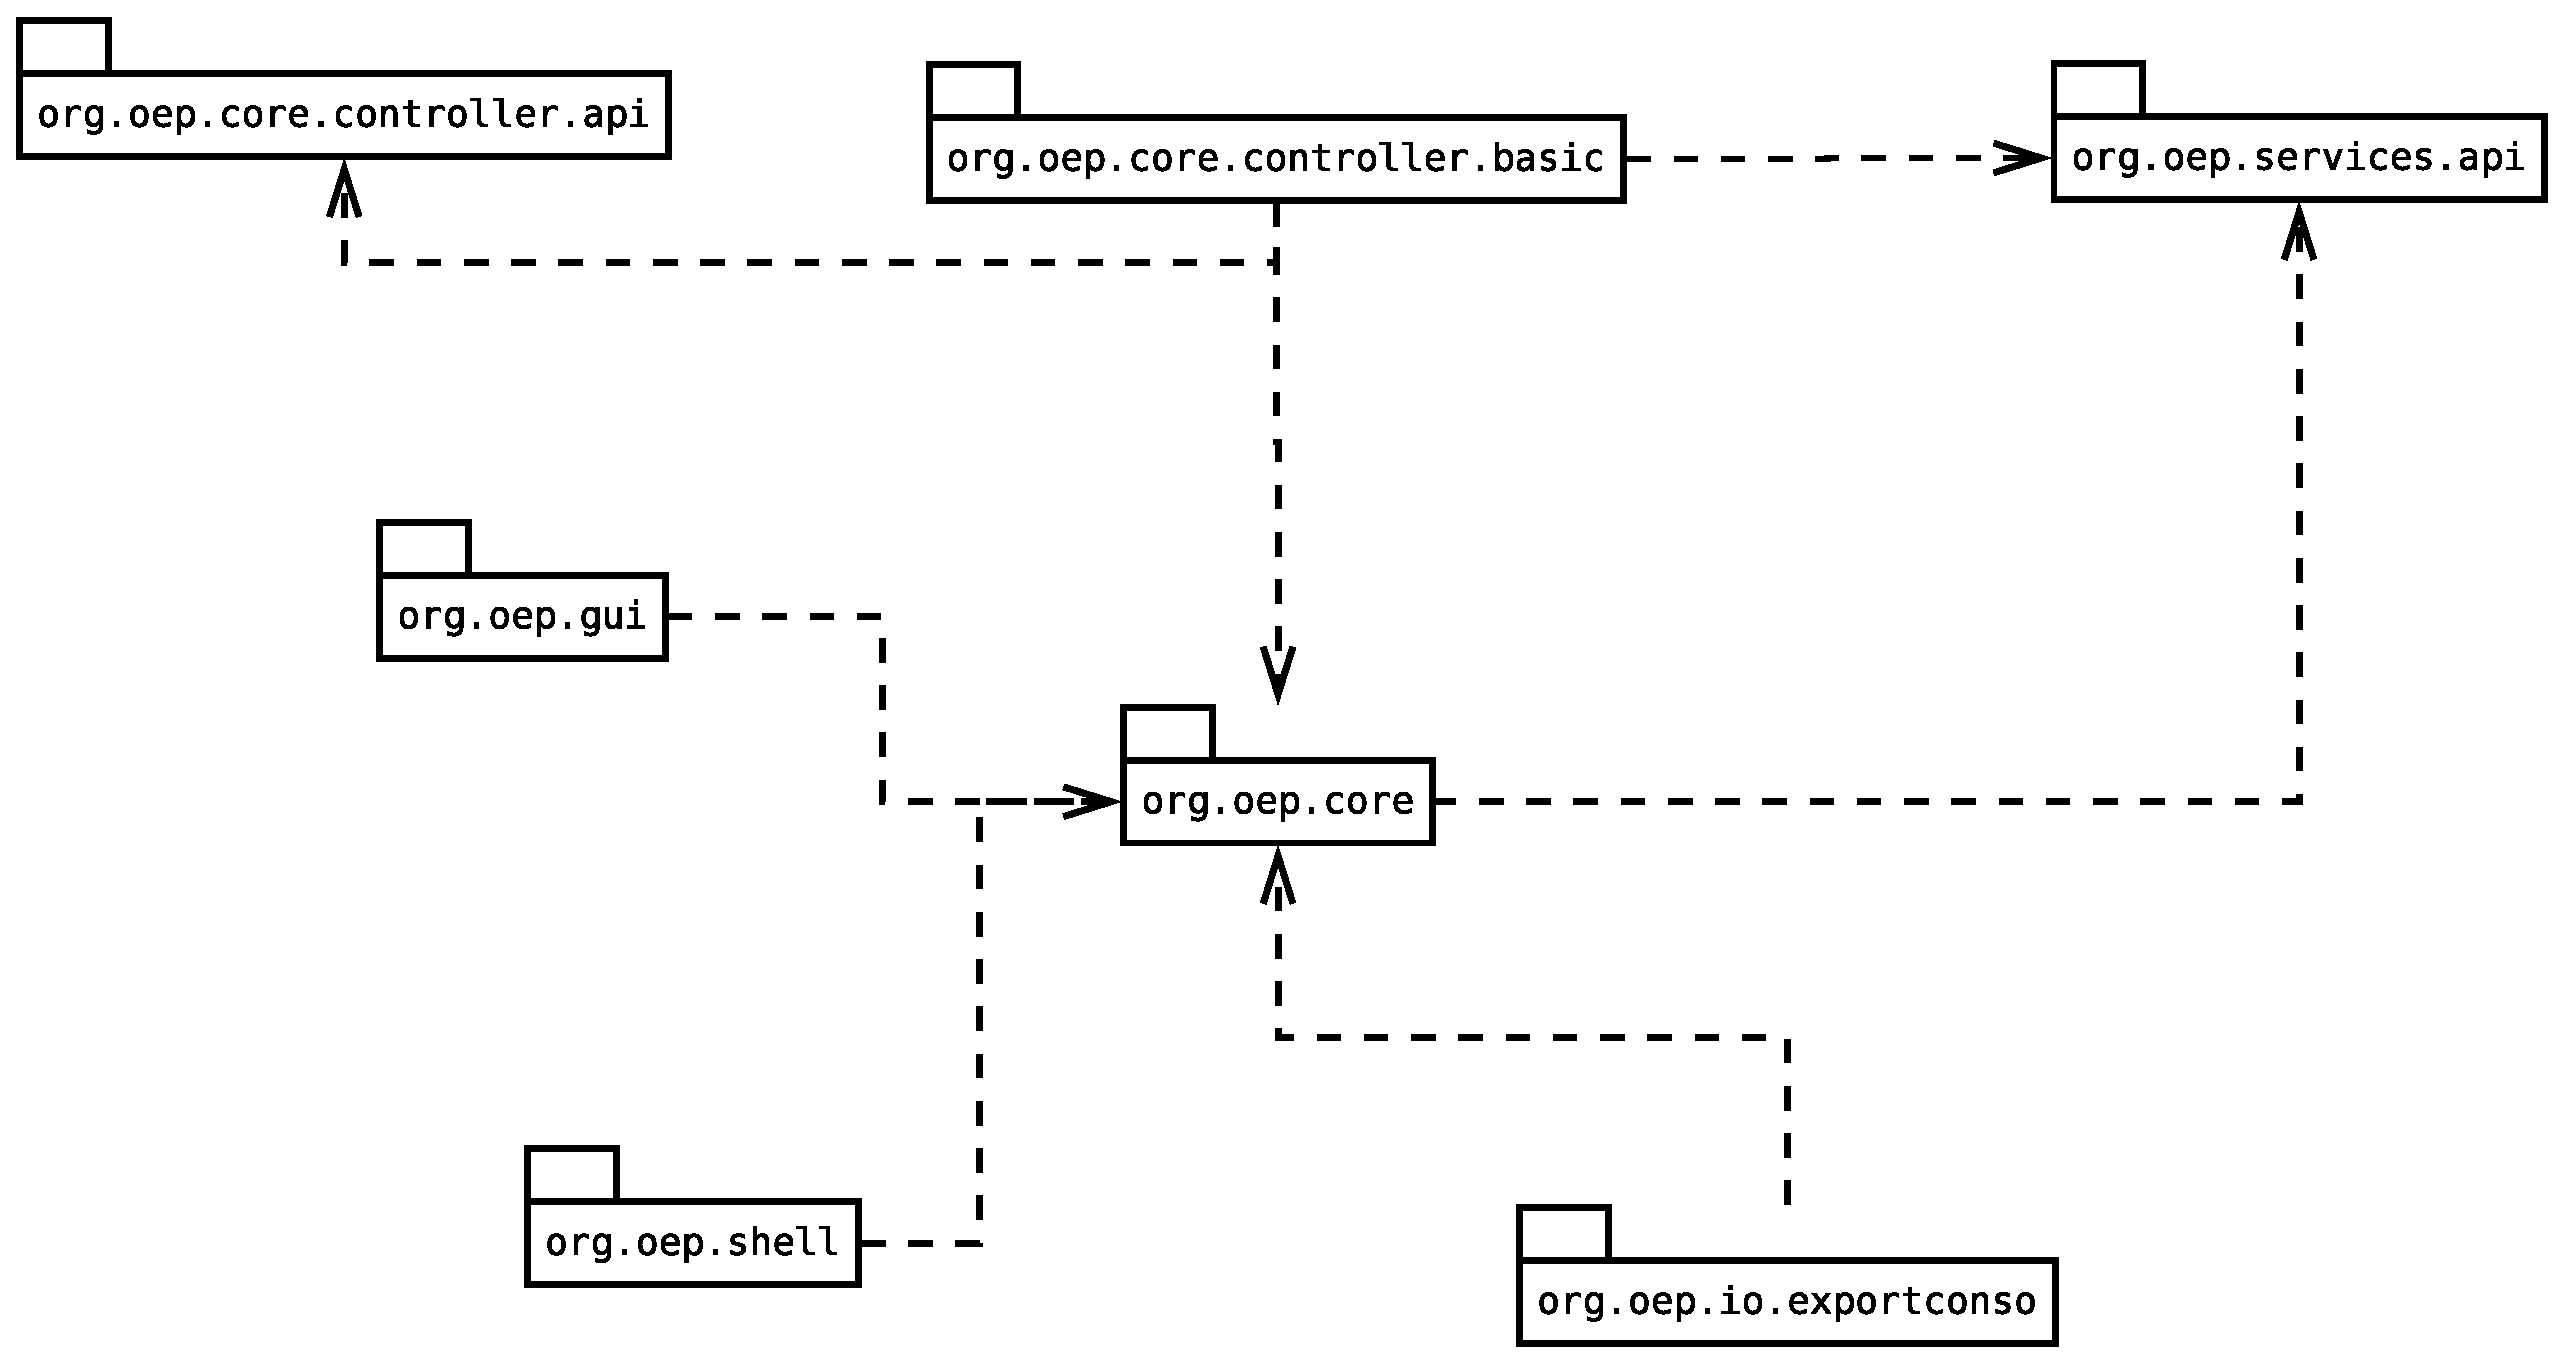
\includegraphics[width=300px]{figures/EcoPattern_Bundle_Diagramme.eps}
		\caption{OSGiEcoPattern : diagramme de liaison des bundles}
	\end{center}
\end{figure}
	\section{Développer une application pour ce framework}
	\section{Un exemple d'application : lecteur audio}

\chapter{Conclusion}
%TODO écrire la conclusion.

\bibliographystyle{plain}
\bibliography{biblio}
\listoffigures{}
\listoftables{}
\appendix

\chapter{Sujet de stage}
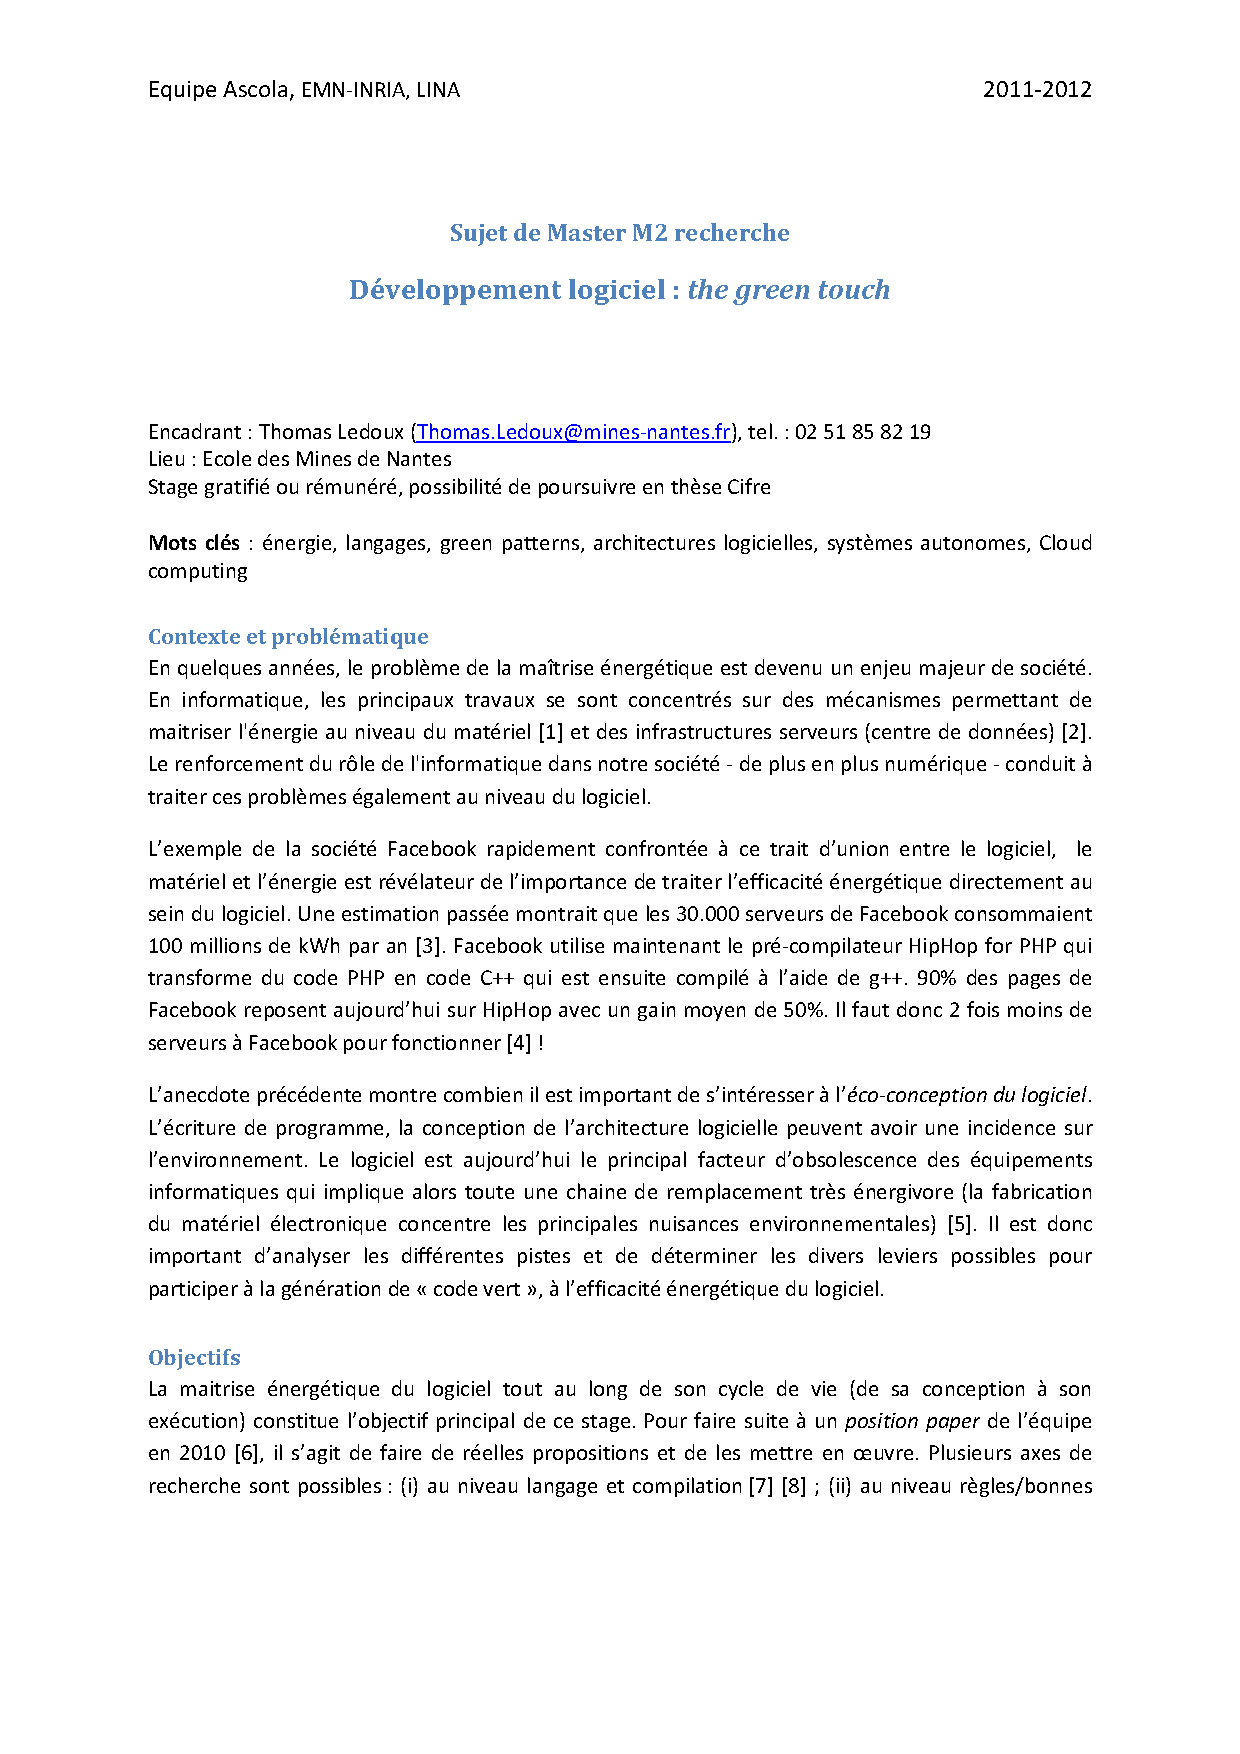
\includepdf[lastpage=3;pages=-]{imports/Sujet_Master_EcoConceptionGL.pdf}

\chapter{Plannification}
%TODO insérer le diagramme de GANT

\end{document}